%%%%%%%%%%%%%%%%%%%%%%%%%%%%%%%%%%%%%%%%%%%%%%%%%%%%%%%%%%%%
%%%%%%%%%%%%%%%%%%%%%%%%%%%%%%%%%%%%%%%%%%%%%%%%%%%%%%%%%%%%
%%%%%%%%%%%%%%%%%%%%%%%%%%%%%%%%%%%%%%%%%%%%%%%%%%%%%%%%%%%%
\section{The DUNE Workflow for Simulations with CAD-Models}\label{Sec:Workflow}
%%%%%%%%%%%%%%%%%%%%%%%%%%%%%%%%%%%%%%%%%%%%%%%%%%%%%%%%%%%%
%%%%%%%%%%%%%%%%%%%%%%%%%%%%%%%%%%%%%%%%%%%%%%%%%%%%%%%%%%%%
%%%%%%%%%%%%%%%%%%%%%%%%%%%%%%%%%%%%%%%%%%%%%%%%%%%%%%%%%%%%

%-------------------------------------------------------------------
\subsection{Overview}
% Bilder
% Tool Chain

\begin{frame}
  \frametitle<presentation>{Overview}
  \textbf{Real world problems can be defined on complex domains.}
  \begin{itemize}
    \item Often, such domains are given by CAD-models.
    \item DUNE cannot handle such models directly.
    \item $\rightarrow$ Need of a workflow to import computational grids
      for CAD-models used in simulations.
  \end{itemize}
  The interface to meshed CAD-Models in DUNE is via \lstinline!Gmsh!-files.
\end{frame}

\begin{frame}
  \frametitle<presentation>{Overview}
  The outline to import meshed CAD-models in DUNE is
  \begin{enumerate}
    \item Create or retrieve a CAD-model.
    \item Edit and mesh the CAD-model with Gmsh
      \href{http://www.geuz.org/msh}{(www.geuz.org/gmsh)}.
    \item Export a \lstinline!.msh!-File from Gmsh.
    \item File can contain additional data such as connected subdomains.
    \item Import the mesh file with the \lstinline!DUNE::GmshReader!.
    \item Evaluate physical data specified in the mesh file.
  \end{enumerate}
  The important steps will be shown in detail in the following sections.
\end{frame}

\begin{frame}
  \frametitle<presentation>{A Meshed CAD-Models Imported to DUNE}
  The picture shows a sample geometry meshed with Gmsh on the left and the mesh
  imported by DUNE on the right.
  %\begin{figure*}
  \begin{center}
    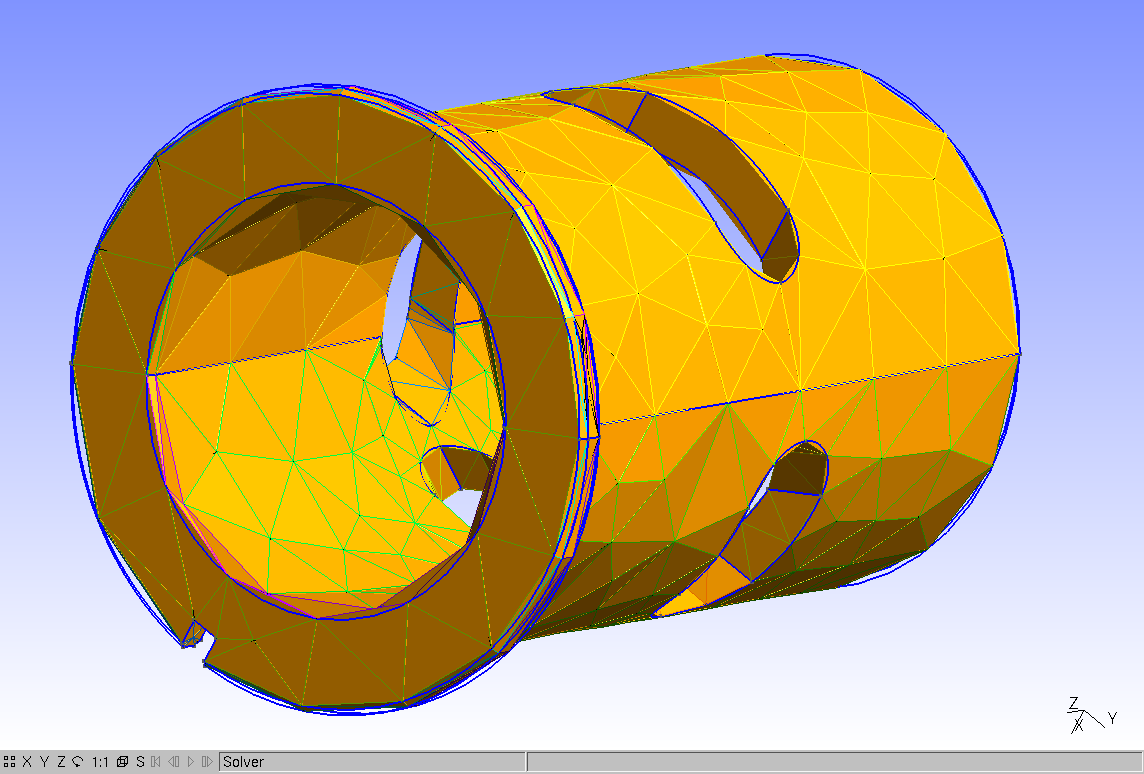
\includegraphics[width=0.48\textwidth]{./EPS/gcad3d_cyl_gmsh}  $\hspace{1mm}$
    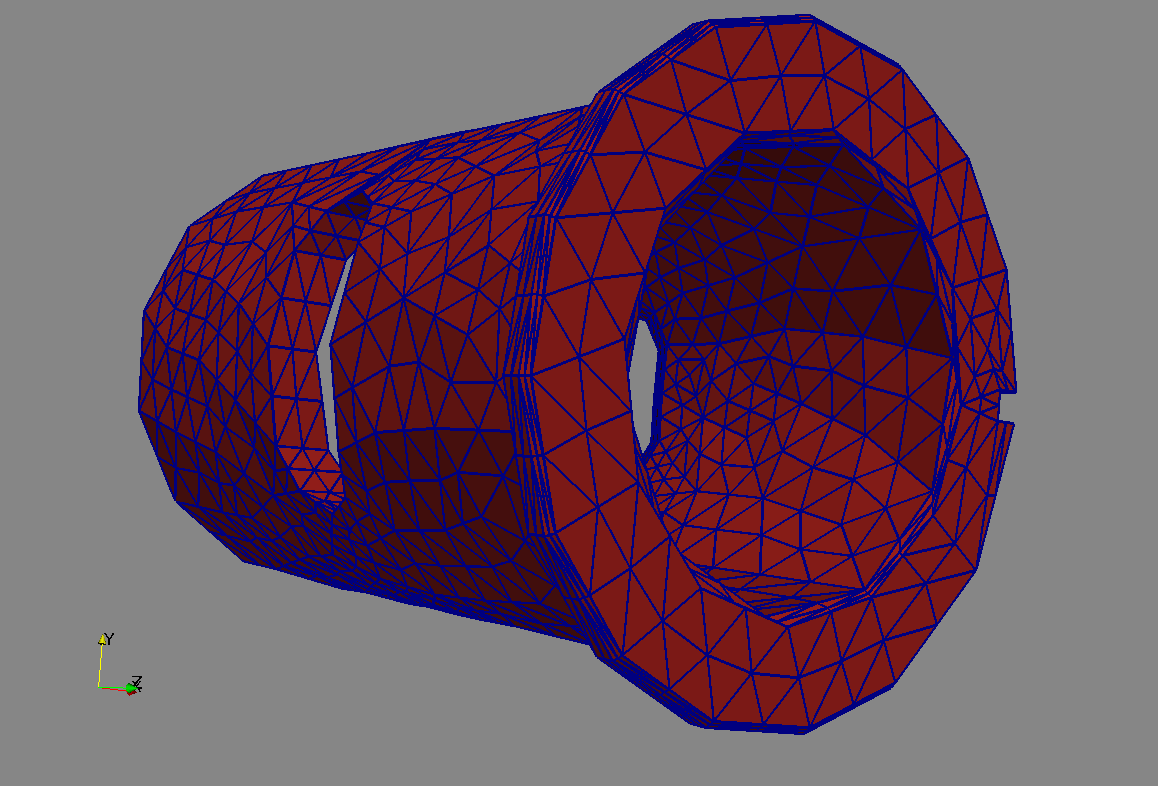
\includegraphics[width=0.48\textwidth]{./EPS/gcad3d_cyl_dune}
    %\caption[]{Some example meshes import to DUNE.}
    %\label{fig:CADExmapleMeshesToDUNE}
  \end{center}
  {\tiny (CAD-Model from gCAD3D).}
  %\end{figure*}
\end{frame}

% tikz style definitions
\mode<all>{
  \tikzstyle{cadsoftware} = [rectangle, draw, fill=blue!30,
      text badly centered, inner sep=0.5em, top color=blue!60]
  \tikzstyle{cadformat} = [rectangle, draw, fill=green!20,
      text badly centered, inner sep=0.56em, top color=orange!50]
}

\begin{frame}
  \frametitle<presentation>{The Workflow to Import meshed CAD-Models to DUNE}
  \begin{figure}[h]
    \begin{center}
      % the flow chart
      \mode<article>{\begin{tikzpicture}}
      \mode<beamer>{\begin{tikzpicture}[scale=0.6] \scriptsize}
        % draw the nodes
        \node [cadsoftware, rectangle split, rectangle split parts=2]
            (dune) at (5, 0) {
              {\Large \textbf{DUNE}}
              \nodepart{second} \texttt{Grid Instance}
            };
        \node [cadsoftware] (gmshreader) at (0, 0) {\texttt{Dune::GmshReader}};
        \node [cadsoftware, rectangle split, rectangle split parts=3]
            (gmsh) at (-4, -4) {
              {\Large \textbf{GMSH}}
              \nodepart{second} Geometry Module
              \nodepart{third}  Mesh Module
            };
        \node [cadformat, rectangle split, rectangle split parts=4]
            (cadformats) at (2, -3.5) {
            \textbf{Geo Formats}
              \nodepart{second} IGES
              \nodepart{third} ACIS
              \nodepart{fourth} STEP
            };
        \node [cadformat, rectangle split, rectangle split parts=3]
            (meshformats) at (2, -7.5) {
              \textbf{Mesh Formats}
              \nodepart{second} UNV
              \nodepart{third} MED
            };
        \node [cadsoftware, rectangle split, rectangle split parts=3]
            (salome) at (7, -6) {
            {\Large \textbf{Salom\'{e}}}
              \nodepart{second} Geometry Module
              \nodepart{third}  Mesh Module
            };
        % draw the connecting arrows
        \path[black!60,->, line width=1.5, shading=axis]
            (cadformats) edge (gmsh.east);
        \path[black!60,->, line width=1.5, shading=axis]
            (meshformats) edge (gmsh.south east);
        \path[black!60,->, line width=1.5, shading=axis]
            (gmshreader.east) edge (dune.195);
        \path[black!60,->, line width=1.5, shading=axis]
            (salome.west) edge (cadformats);
        \path[black!60,->, line width=1.5, shading=axis]
            (salome.205) edge (meshformats.east);
        \path[black!60,->, line width=1.5, shading=axis]
            (gmsh.205) edge [out= 180, in= 180] (gmshreader.west);
      \end{tikzpicture}
    \end{center}
  \end{figure}
  The flow charts depicts the general way of using gmsh or another external
  geometry modeler behind it to import CAD-models meshed by Gmsh into DUNE.
\end{frame}

%-------------------------------------------------------------------
\subsection{Gmsh and the DUNE Gmsh-Interface}
% DUNE GmshReader
% Gmsh und OpenCascade
% Installation
% welche Grids?

\begin{frame}[fragile,allowframebreaks,allowdisplaybreaks]
  \frametitle{The Dune::GmshReader}
  We begin with the import of a Mesh file \lstinline!meshfile.msh! using DUNE's
  \lstinline!GmshReader!:
  \lstinputlisting[basicstyle=\tiny,numbers=left,
      numberstyle=\tiny, numbersep=2pt]{./src_examples/gridtest.cc}
      \textbf{Changes to the code seen up to now are:}
  \begin{itemize}
    \item Include the Gmsh-Interface header from \lstinline!dune-grid! (line
      $12$).
    \item Use \lstinline!UGGrid! -- Up to now \lstinline!UGGrid! and
      \lstinline!ALUGrid! are feasible for Gmsh meshes (line $33$-$35$).
    \item Import gmsh file (line $37$-$40$).
  \end{itemize}
\end{frame}

\begin{frame}[fragile,allowframebreaks,allowdisplaybreaks]
  \frametitle{Gmsh}
  The mesh-files are created and exported by the exported software \emph{Gmsh},
  which is able to
  \begin{itemize}
    \item Import CAD models in various formats
      (\lstinline!GEO, STEP, IGES, BREP, ACIS, ...!),
    \item Group subdomains of the models into phyiscal \emph{entities} or
      \lstinline{groups},
    \item Mesh the models,
    \item Write the meshes including physical group regions to a mesh file
      (file-ending \lstinline!.msh!).
  \end{itemize}
  \pagebreak<presentation>
  It comes with a more or less user-friedly GUI:
  \begin{center}
    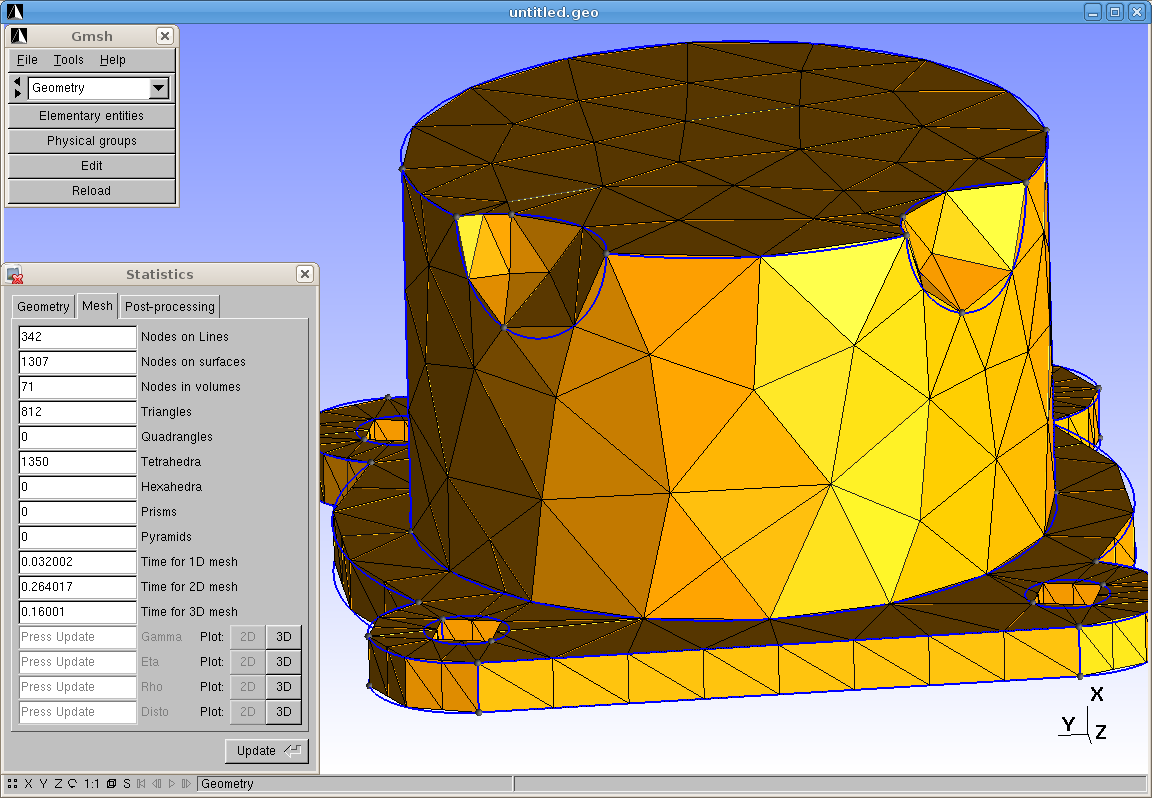
\includegraphics[width=0.7\textwidth]{./EPS/gcad3d_deckel}
  \end{center}
  {\tiny (CAD-Model from gCAD3D).}

  \textbf{Further features of Gmsh:}
  \begin{itemize}
    \item Geometry Kernel: OpenCascade
      \begin{itemize}
        \item Gmsh $\leq$ 2.3.1:\\ Build from scratch for OpenCascde and Gmsh
          necessary to import CAD-models.
        \item Gmsh $\geq$ 2.4.2:\\ Precompiled build for Linux and MAC work with
          OpenCascade packages from distributor (Tested for Debian and MacOS).
      \end{itemize}
    \item Does not cover full functionality of geometry kernel.
  \end{itemize}
\end{frame}

\subsubsection*{Further notes on ineraction between DUNE and Gmsh}

\begin{frame}
  \frametitle{DUNE and Gmsh Notes}
  \begin{itemize}
    \item Possible: Second order boundary representation, readable by the
      GmshReader (Instable in the current trunk!).
    \item Underlying DUNE-Grid needs to support higher order boundaries. During grid
      refinement boundary is approximated the better.
    \item In DUNE: Higher order local FE bases available.
    \item Higher order elements are generally possible but not
      implemented yet in DUNE:
      \begin{itemize}
        \item Need approriate grid-managers.
        \item Need mesher which exports such elements.
        \item GmshReader uses \emph{GridFactories} to create grids.
          \begin{itemize}
            \item GridFactory implementation depends on DUNE GridType.
            \item For UG and ALU the Factories are ready.
            \item For other grids, user may need to implement a specific factory.
          \end{itemize}
      \end{itemize}
  \end{itemize}
\end{frame}

%-------------------------------------------------------------------
\subsection{Importing and Meshing CAD-Geometries with Gmsh}
% CAD-Files Uebersicht
% install with opencascade
% Import
% Welcher Mesher?

\begin{frame}
  \frametitle{Common CAD-File Formats Readable by Gmsh}
  \textbf{Gmsh allows to import CAD-models in common formats:}
  \begin{center}
    \begin{tabular}{|l|l|l|}
      \hline
      Format & Ending & Description
      \\
      \hline
      \hline
      STEP & \lstinline!.stp, .step! & ISO10303 norm, STandard for the\\
      & & Exchange of Product model data.
      \\
      \hline
      IGES & \lstinline!.igs, .iges! & Transfers mainly geometry data\\
      & & 2D/3D shape models (NURBS, Bezier, \ldots)
      \\
      \hline
      ACIS & \lstinline!.sat! & Volume modelling kernel. Widely used format.
      \\
      \hline
      BREP & \lstinline!.brp! & List of convex polygons consisting of point lists\\
      & & In OpenCascade very limited!
      \\
      \hline
      GEO & \lstinline!.geo! & The native Gmsh geometry format.
      \\
      \hline
    \end{tabular}
  \end{center}
\end{frame}

\begin{frame}
  \frametitle{Meshing CAD-Models with Gmsh}
  \textbf{Gmsh comes with a meshing functionality:}
  \begin{itemize}
    \item Advancing front, and
    \item Delaunay meshes.
    \item Meshers can be parametrized by hypothesises.
    \item All meshes are handled as unstructured grids.
    \item Only simplicial meshes.
  \end{itemize}
\end{frame}

%-------------------------------------------------------------------
\subsection{Attaching Data to a CAD-Geometry and its Mesh}
% Gruppen in Gmsh
% Gmshreader nur eine Gruppe pro Element!
% PDELab-Code

\begin{frame}[fragile,allowframebreaks,allowdisplaybreaks]
  \frametitle<presentation>{Physical Groups in CAD-Models}
  \begin{minipage}{0.67\linewidth}
    \textbf{Parameters can be associated to subdomains of the
    domain, e.g.}
    \begin{itemize}
      \item Material properties (conductivities,\ldots),
      \item Boundary conditions,
      \item \ldots
    \end{itemize}
    \textbf{The subdomains available in Gmsh are:}
    \begin{itemize}
      \item Volume groups,
      \item Surface groups,
      \item Line groups,
      \item Point groups.
    \end{itemize}
    \textbf{How to set groups:}
    \begin{itemize}
      \item Via \texttt{Geometry} $\rightarrow$ \texttt{Physical groups} in
        the menu window.
    \end{itemize}
  \end{minipage}
  \hfill
  \begin{minipage}{0.31\linewidth}
    \begin{center}
      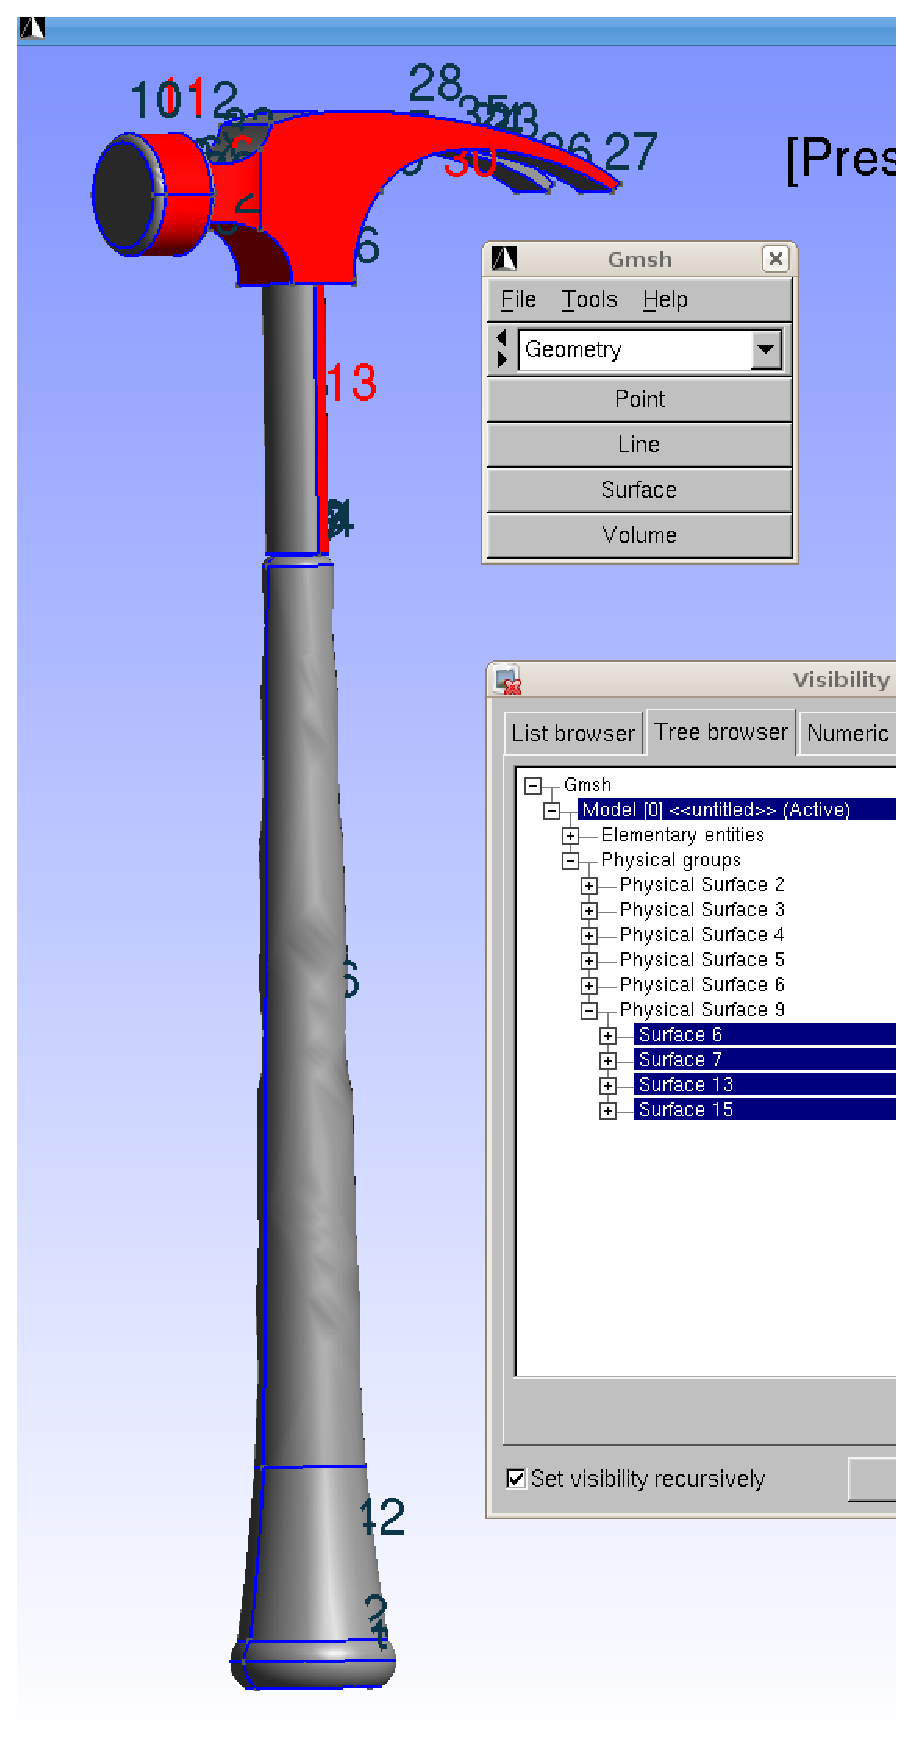
\includegraphics[width=\linewidth]{./EPS/hammer_surfgroups}
    \end{center}
  \end{minipage}
\end{frame}

\begin{frame}
  \frametitle<presentation>{Evaluating Physical Groups with the GmshReader}
  The \lstinline!Dune::GmshReader! is able to read
  \begin{itemize}
    \item Volume groups, and
    \item Surface groups
  \end{itemize}
  from a \lstinline!.msh!-file. Mappings
  \begin{itemize}
    \item Codim 0 entities $\Leftrightarrow$ Geometry volume groups, and
    \item Codim 1 entities $\Leftrightarrow$ Geometry surface groups,
  \end{itemize}
  can be saved in two \lstinline!std::vector<int>!s.
\end{frame}

\begin{frame}[fragile,allowframebreaks,allowdisplaybreaks]
  \frametitle<presentation>{An Example for Physical Grouping in Gmsh}
  The next picture shows physical surface groups set by user interaction:

  \begin{minipage}{\linewidth}
    \begin{minipage}{0.64\linewidth}
      \begin{center}
        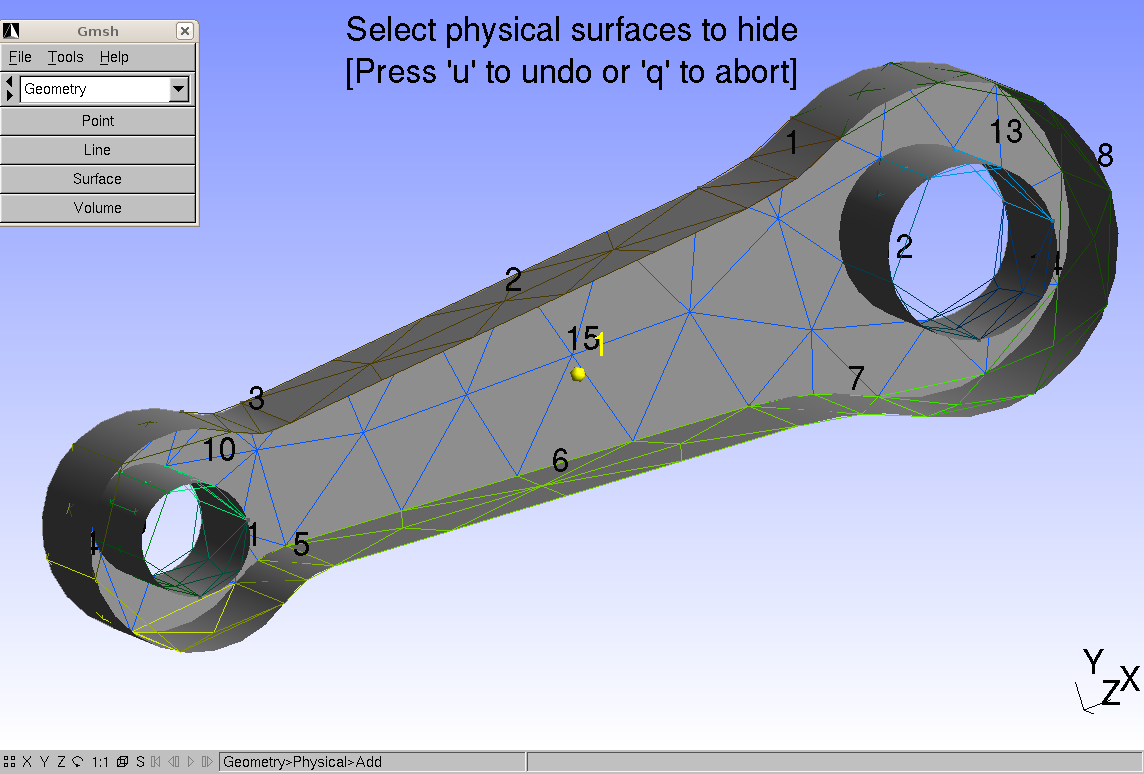
\includegraphics[width=\textwidth]{./EPS/crank/crank_surfgroups1}
      \end{center}
    \end{minipage}
    \hfill
    \begin{minipage}{0.35\linewidth}
      \begin{center}
        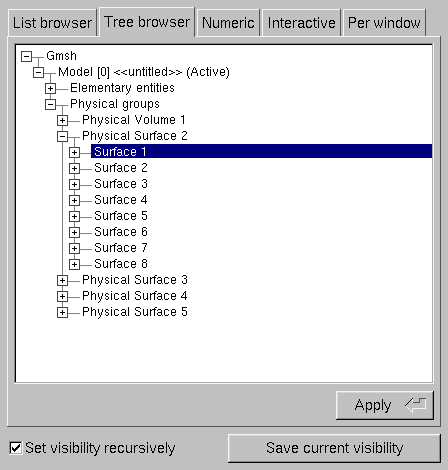
\includegraphics[width=\textwidth]{./EPS/crank/crank_surfgroups2}
      \end{center}
    \end{minipage}
  \end{minipage}
\end{frame}

\begin{frame}[fragile,allowframebreaks,allowdisplaybreaks]
  \frametitle<presentation>{The example mesh read by GmshReader in Dune}
  \begin{center}
    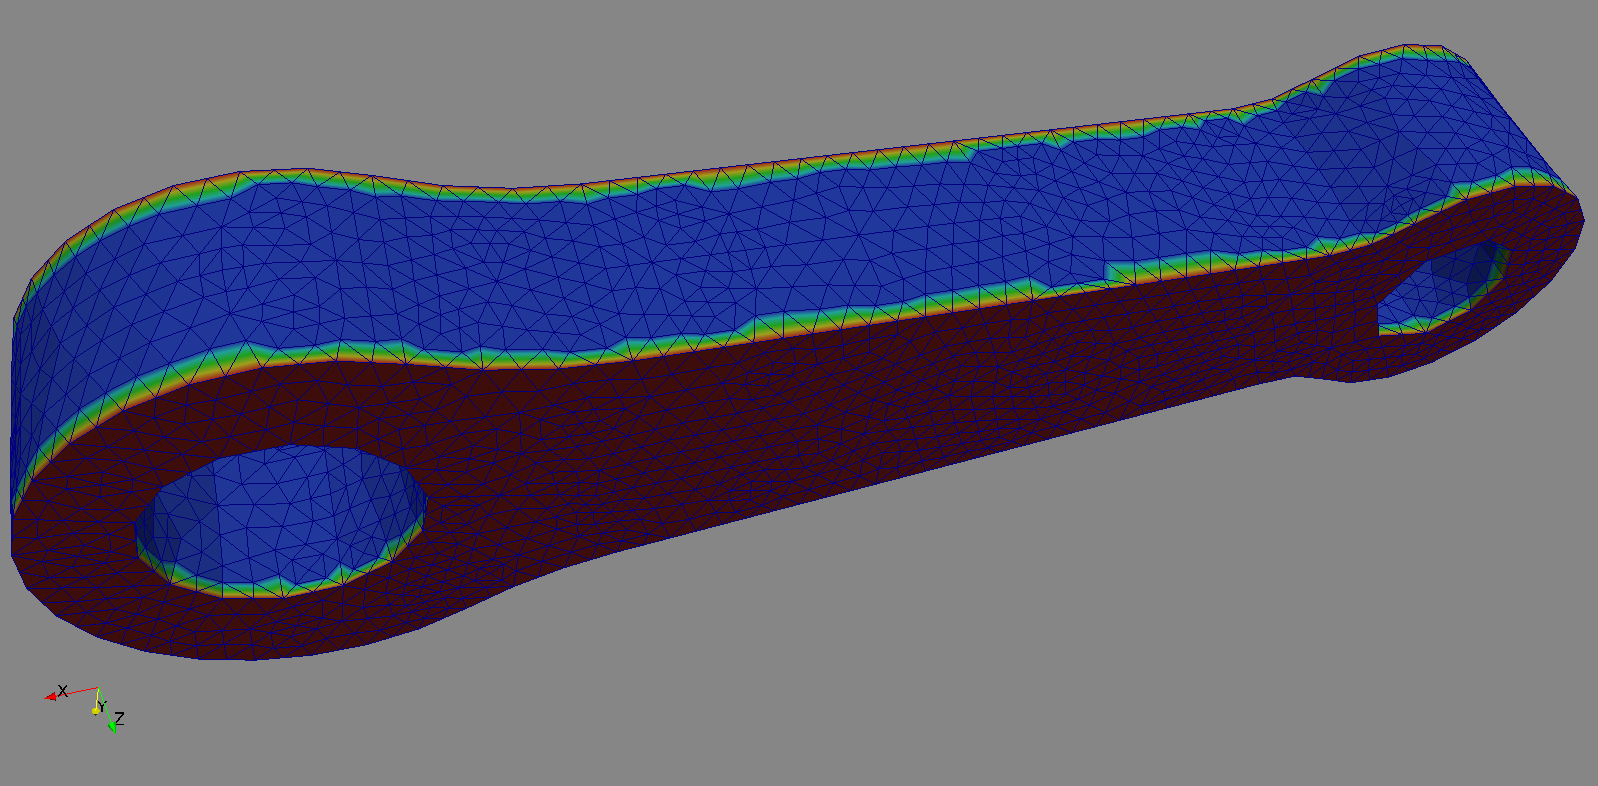
\includegraphics[width=0.7\textwidth]{./EPS/crank/crank_DirBC}
  \end{center}
  This above picture shows the mesh read by the GmshReader. Dirichlet constraints are
  set by the \lstinline!set_constrained_dofs! method in Dune (red colored
  faces). Remaining faces have Neumann-0 boundary conditions.
\end{frame}

%-------------------------------------------------------------------
\subsection{A sample DUNE-Simulation importing a CAD-model}

\begin{frame}<presentation>[fragile,allowframebreaks,allowdisplaybreaks]
  \frametitle{Using Physical Groups from within DUNE}
  \textbf{Next we solve the constraint stationary linear diffusion problem
  (cf. 1st lecture) on the crank-domain. Possible changes are}:
  \begin{itemize}
    \item Use \lstinline!Dune::GmshReader! and \lstinline!UGGrid!,
    \item Use $P1$-elements,
    \item Rewrite
      \begin{itemize}
        \item \lstinline!bctype.hh!,
        \item \lstinline!bcextension.hh!,
        \item Source term evaluation,
        \item Diffusion parameter evaluation.
      \end{itemize}
      \textbf{Boundary conditions and material parameters may depend on physical group
      maps now.}
    \item The PDELab-LocalOperator is parametrized with boundary selection and value
      classes, a source term class and a class for the non-constant material
      parameter.
  \end{itemize}
  \textbf{The Code constist of four files:}
  \begin{itemize}
    \item \lstinline!cadsample.cc!:\\ Main file creating grid files from Gmsh files,
    \item \lstinline!cadsample_parameter.hh!:\\ Parameter classes which contain maps to
      physical groups,
    \item \lstinline!cadsample_P1.hh!:\\ Set up the P1 driver,
    \item \lstinline!cadsample_operator.hh!:\\ The local operator parametrized by the
      classes from \lstinline!cadsample_parameter.hh!
  \end{itemize}
\end{frame}

\begin{frame}<presentation>[fragile,allowframebreaks,allowdisplaybreaks]
  \frametitle<presentation>{The Main File of the Example}
  \lstinputlisting[basicstyle=\tiny,numbers=left,firstline=53,lastline=122,firstnumber=53,
      numberstyle=\tiny, numbersep=2pt]{./src_examples/cadsample.cc}
  \textbf{Notes:}
  \begin{itemize}
    \item In line $75$, the \lstinline!GmshReader! takes two vectors
      (instantiated in lines $69,70$) to store volume and surface map data from
      the Gmsh file.
    \item In line $85-97$, the parameter classes for the problem are created.
      In the constructor they take the according vectors.\\
      Example: \lstinline!CrankBCType! evaluates the mapping \lstinline!Dune::Intersection!
      with boundary to physical group of geometrical boundary.
    \item All parameter objects are passed to the driving function
      \lstinline!cadsample_P1! in line $111$ which forwards them to the operator.
  \end{itemize}
\end{frame}
\mode<article>{
  \begin{Lst} \mbox
  \nopagebreak
  \lstinputlisting[basicstyle=\scriptsize,numbers=left,
      numberstyle=\tiny, numbersep=2pt]{./src_examples/cadsample.cc}
  \end{Lst}
  \textbf{Notes:}
  \begin{itemize}
    \item The \lstinline!GmshReader! takes two vectors to store volume and surface
      map data from the Gmsh file.
    \item In function \lstinline!crank!, the parameter classes for the problem are created.
      In the constructor they take the according vectors.\\
      Example: \lstinline!CrankBCType! evaluates the mapping \lstinline!Dune::Intersection!
      with boundary to physical group of geometrical boundary.
    \item All parameter objects are passed to the driving function
      \lstinline!cadsample_P1! which forwards them to the operator.
  \end{itemize}
}

\begin{frame}<presentation>[fragile,allowframebreaks,allowdisplaybreaks]
  \frametitle<presentation>{The Parameter Classes in Detail}
  \lstinputlisting[basicstyle=\tiny,numbers=left,linerange={19-61,63-115,120-158,161-189},
      numberstyle=\tiny, numbersep=2pt]{./src_examples/cadsample_parameter.hh}
  \textbf{Notes:}
  \begin{itemize}
    \item The parameter classes evaluate the physical maps instead of global
      coordinates now.
    \item E.g., take the diffusion coefficient. Based on the element index
      it evaluates the physical group map for volumes.
    \item Similar evaluation for the other parameter classes.
  \end{itemize}
\end{frame}
\mode<article>{
  \begin{Lst} \mbox
  \nopagebreak
  \lstinputlisting[basicstyle=\scriptsize,numbers=left,
      numberstyle=\tiny, numbersep=2pt]{./src_examples/cadsample_parameter.hh}
  \end{Lst}
  \textbf{Notes:}
  \begin{itemize}
    \item The parameter classes evaluate the physical maps instead of global
      coordinates now.
    \item E.g., take the diffusion coefficient. Based on the element index
      it evaluates the physical group map for volumes.
    \item Similar evaluates hold true for the other parameter classes.
  \end{itemize}
}

\begin{frame}<presentation>[fragile,allowframebreaks,allowdisplaybreaks]
  \frametitle<presentation>{The Driver function for the Example}
  \lstinputlisting[basicstyle=\tiny,numbers=left,linerange={1-6,27-34},
      numberstyle=\tiny, numbersep=2pt]{./src_examples/cadsample_P1.hh}
  \textbf{Notes:}
  \begin{itemize}
    \item The driver is nearly unchanged to the stationary examples.
    \item Passes the parameter objects to the operator and constraints.
  \end{itemize}
\end{frame}
\mode<article>{
  \begin{Lst} \mbox
  \nopagebreak
  \lstinputlisting[basicstyle=\scriptsize,numbers=left,
      numberstyle=\tiny, numbersep=2pt]{./src_examples/cadsample_P1.hh}
  \end{Lst}
  \textbf{Notes:}
  \begin{itemize}
    \item The driver is nearly unchanged to the stationary examples.
    \item Passes the parameter objects to the operator and constraints.
  \end{itemize}
}

\begin{frame}<presentation>[fragile,allowframebreaks,allowdisplaybreaks]
  \frametitle<presentation>{The Parametrized Local Operator for the Example}
  \lstinputlisting[basicstyle=\tiny,numbers=left,
      linerange={7-22,40-47,96-105,113-117,155-158,166-171},
      numberstyle=\tiny, numbersep=2pt]{./src_examples/cadsample_operator.hh}
  \textbf{Notes:}
  \begin{itemize}
    \item Operator is parametrized with boundary type selection,
      boundary extension and boundary flux classes.
    \item Source term vanishes but could also be a parameter to the operator.
    \item Compare Evaluation of the parameters to the parameter classes!
  \end{itemize}
\end{frame}
\mode<article>{
  \begin{Lst} \mbox
  \nopagebreak
  \lstinputlisting[basicstyle=\scriptsize,numbers=left,
      numberstyle=\tiny, numbersep=2pt]{./src_examples/cadsample_operator.hh}
  \end{Lst}
  \textbf{Notes:}
  \begin{itemize}
    \item The operator is now parametrized with the boundary type selection,
      boundary extension and boundary flux classes.
    \item Source term vanishes but could also be a paramter to the operator.
    \item Evaluation of the parameter in operator via enities and intersecions.
      Compare the parameter classes!
  \end{itemize}
}

\begin{frame}
  \frametitle<presentation>{Simulation results}
  \begin{center}
    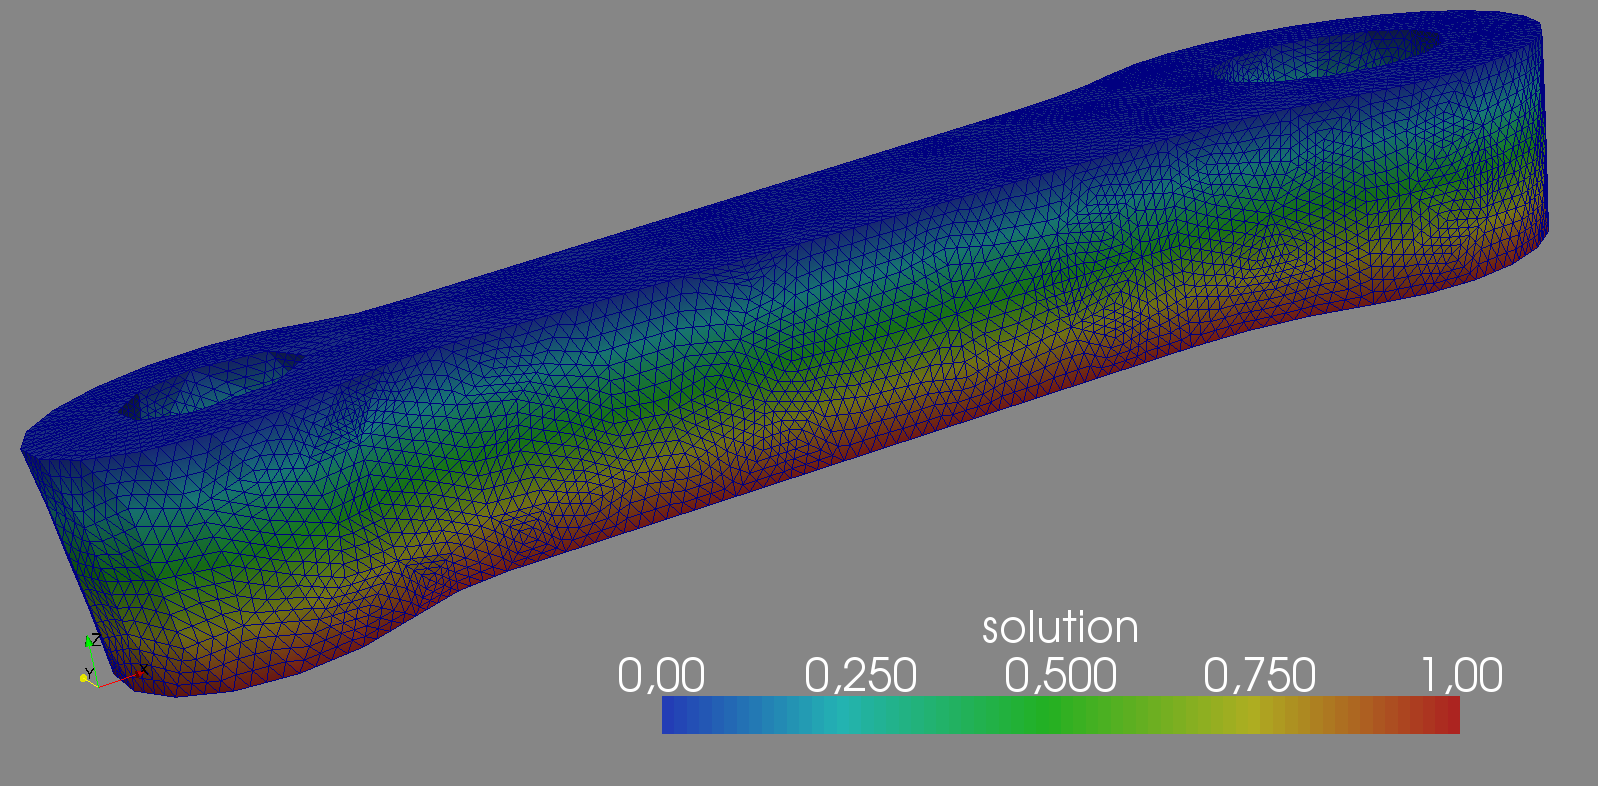
\includegraphics[width=0.7\textwidth]{./EPS/crank/crank_sol}
  \end{center}
  This picture shows the results of the simulation (stationary diffusion, no flux
  boundaries, P1-FEM).
\end{frame}

%-------------------------------------------------------------------
\subsection{Some other applicable Open Source CAD-Tools}

% Constructing Geometries
% Export von geo und unv
% Ausblick: Reader
\begin{frame}
  \frametitle{Salome}
  \textbf{Salome is a more user-friendly CAE-environment which can also export
  CAD-models and meshes suitable for Gmsh-Import}.
  \begin{itemize}
    \item Geometry Kernel: OpenCascade, exposes more of the functionality than Gmsh.
    \item Can import and export IGES-, STEP-, BREP-, ACIS-files.
    \item Can import and export STL and UNV-meshes.
    \item Has a generic Mesher interface (Available: Netgen, GHS3D, ...)
    \item User friendly GUI for creating and processing CAD-models.
  \end{itemize}
  \mode<presentation>{$\longrightarrow$ We will use it in the exercises.}
\end{frame}

\begin{frame}
  \frametitle{Other Open Source CAD-Tools}
  %\begin{table}
    Some other CAD-Tools which are able to export geometry models or mesh
    files suitable for Gmsh import:
    \begin{center}
      \small
      \begin{tabular}{|c|c|c|c|c|c|}
        \hline
        Tool & Licence & Geom & Geom & Mesh
        \\
        &  & Import & Import & Export
        \\
        \hline
        \hline
        Gmsh & LGPL & geo & iges, step, brep, acis & msh
        \\
        \hline
        Salome & LGPL & iges, step, brep, acis & iges, step, brep, acis & unv,
        stl
        \\
        \hline
        gCAD3D & Freeware & step, iges & step, iges &
        \\
        \hline
        Blender & own (BL) & CSG & iges &
        \\
        \hline
        PythonOCC & GPL & \multicolumn{2}{c}{Python-Wrapper for OpenCascade} &
        \\
        \hline
      \end{tabular}
      %\caption{Some CAD tools.}
      %\label{tab:CADTools}
    \end{center}
  %\end{table}
\end{frame}

\cleardoublepage
